\section{Bestrahlungsplanung}
\label{sec:Bestrahlungsplanung}

Bevor mit dem Erstellen des Bestrahlungsplanes begonnen wird, wird zunächst der gesamte Kopf, der auf dem CT-Aufnahmen abgebildet ist, konturiert.
Bei dieser Bestrahlung müssen außerdem Risikoorgane in das CT-Bild eingezeichnet werden. Zu den
Risikoorganen gehören das Chiasma, die Augenlinsen und die gesamten Augen. Für diese
Bestrahlung werden zwei Felder verwendet, die eine Gantry-Rotation von $80°$ und $275°$ haben. Beide Felder haben eine Größe von $20$ x $\SI{18.4}{\centi\meter\squared}$ und sind auch gleich auf $50\%$ gewichtet. Damit die Augenlinsen vor der Strahlung geschützt werden,
werden bei beiden Feldern MLCs verwendet. Die Einstellungen der MLCs ist in Abbildung \ref{abb:MLC} dargestellt.
Außerdem ist der Plan auf \enquote{$100\%$ target mean} normiert worden.

\begin{figure}[H]
  \centering
  \begin{subfigure}{\textwidth}
    \centering
    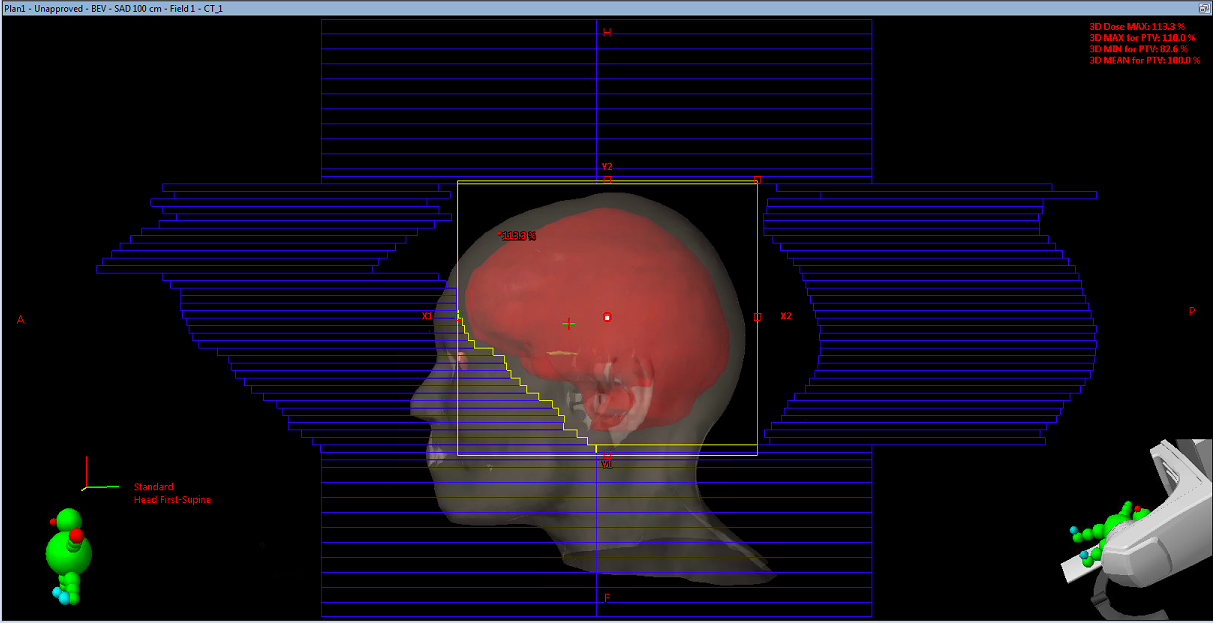
\includegraphics[height = 5cm]{Bilder/MLC_Feld1.png}
    \caption{}
  \end{subfigure}
  \begin{subfigure}{\textwidth}
    \centering
    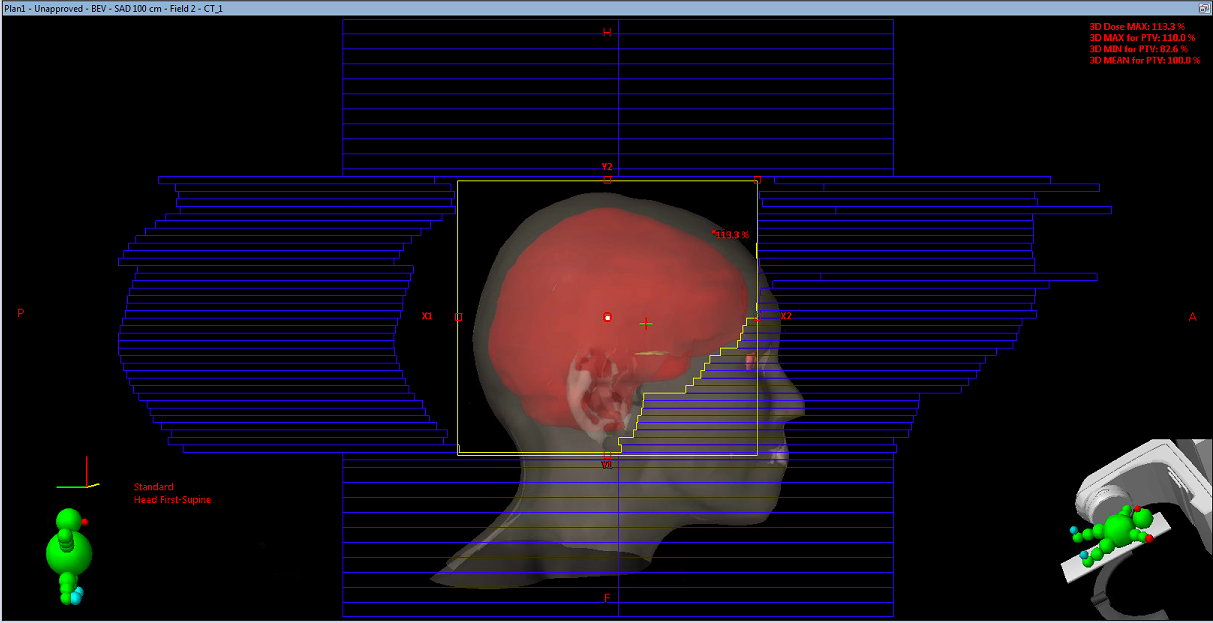
\includegraphics[height=5cm]{Bilder/MLC_Feld2.png}
    \caption{}
  \end{subfigure}
  \caption{Darstellung der Lamellenpositionen der beiden Felder. Bei a) die Positionen bei dem Feld bei $80°$ und bei b) die Positionen bei dem Feld bei $275°$.}
  \label{abb:MLC}
\end{figure}
